\section{GtkApplication and
GtkApplicationWindow}\label{gtkapplication-and-gtkapplicationwindow}

\subsection{GtkApplication}\label{gtkapplication}

\subsubsection{GtkApplication and
g\_application\_run}\label{gtkapplication-and-g_application_run}

People write programming codes to make an application. What are
applications? Applications are software that runs using libraries, which
are the OS, frameworks and so on. In GTK 4 programming, the
GtkApplication is a program (or executable) that runs using Gtk
libraries.

The basic way to write a GtkApplication is as follows.

\begin{itemize}
\tightlist
\item
  Create a GtkApplication instance.
\item
  Run the application.
\end{itemize}

That's all. Very simple. The following is the C code representing the
scenario above.

\begin{lstlisting}[language=C, numbers=left]
#include <gtk/gtk.h>

int
main (int argc, char **argv) {
  GtkApplication *app;
  int stat;

  app = gtk_application_new ("com.github.ToshioCP.pr1", G_APPLICATION_DEFAULT_FLAGS);
  stat =g_application_run (G_APPLICATION (app), argc, argv);
  g_object_unref (app);
  return stat;
}
\end{lstlisting}

The first line says that this program includes the header files of the
Gtk libraries. The function \passthrough{\lstinline!main!} is a startup
function in C language. The variable \passthrough{\lstinline!app!} is
defined as a pointer to a GtkApplication instance. The function
\passthrough{\lstinline!gtk\_application\_new!} creates a GtkApplication
instance and returns a pointer to the instance. The GtkApplication
instance is a C structure data in which the information of the
application is stored. The arguments will be explained later. The
function \passthrough{\lstinline!g\_application\_run!} runs an
application that the instance defined. (We often say that the function
runs \passthrough{\lstinline!app!}. Actually,
\passthrough{\lstinline!app!} is not an application but a pointer to the
instance of the application. However, it is simple and short, and
probably no confusion occurs.)

Here I used the word \passthrough{\lstinline!instance!}. Instance, class
and object are terminologies in Object Oriented Programming. I use these
words in the same way. But, I will often use ``object'' instead of
``instance'' in this tutorial. That means ``object'' and ``instance'' is
the same. Object is a bit ambiguous word. In a broad sense, object has
wider meaning than instance. So, readers should be careful of the
contexts to find the meaning of ``object''. In many cases, object and
instance are interchangeable.

The function \passthrough{\lstinline!gtk\_application\_new!} has two
parameters.

\begin{itemize}
\item
  Application ID (com.github.ToshioCP.pr1). It is used to distinguish
  applications by the system. The format is reverse-DNS. See
  \href{https://developer.gnome.org/documentation/tutorials/application-id.html}{GNOME
  Developer Documentation -- Application ID} for further information.
\item
  Application flag (G\_APPLICATION\_DEFAULT\_FLAGS). If the application
  runs without any arguments, the flag is
  G\_APPLICATION\_DEFAULT\_FLAGS. Otherwise, you need other flags. See
  \href{https://docs.gtk.org/gio/flags.ApplicationFlags.html}{GIO API
  reference} for further information.
\end{itemize}

Notice: If your GLib-2.0 version is older than 2.74, use
\passthrough{\lstinline!G\_APPLICATION\_FLAGS\_NONE!} instead of
\passthrough{\lstinline!G\_APPLICATION\_DEFAULT\_FLAGS!}. It is an old
flag replaced by
\passthrough{\lstinline!G\_APPLICATION\_DEFAULT\_FLAGS!} and deprecated
since version 2.74.

To compile this, run the following command. The string
\passthrough{\lstinline!pr1.c!} is the filename of the C source code
above.

If you've downloaded this repository, you don't need to create the file.
There's the same file at \passthrough{\lstinline!src/misc/pr1.c!} in
your local repository. All the example codes are under the
\passthrough{\lstinline!src!} directory as well.

\begin{lstlisting}
$ gcc `pkg-config --cflags gtk4` pr1.c `pkg-config --libs gtk4`
\end{lstlisting}

The C compiler gcc generates an executable file,
\passthrough{\lstinline!a.out!}. Let's run it.

\begin{lstlisting}
$ ./a.out

(a.out:5084): GLib-GIO-WARNING **: 09:52:04.236: Your application does not implement
g_application_activate() and has no handlers connected to the 'activate' signal.
It should do one of these.
$
\end{lstlisting}

Oh, it just produces an error message. This error message shows that the
GtkApplication object ran, without a doubt. Now, let's think about what
this message means.

\subsubsection{Signals}\label{signals}

The message tells us that:

\begin{enumerate}
\def\labelenumi{\arabic{enumi}.}
\tightlist
\item
  The application doesn't implement
  \passthrough{\lstinline!g\_application\_activate()!},
\item
  It has no handlers connected to the ``activate'' signal, and
\item
  You will need to solve at least one of these.
\end{enumerate}

These two problems are related to signals. So, I will explain that
first.

A signal is emitted when something happens. For example, a window is
created, a window is destroyed and so on. The signal ``activate'' is
emitted when the application is activated. (Activated is a bit different
from started, but you can think of them both as almost the same so far.)
If the signal is connected to a function, which is called a signal
handler or simply handler, then the function is invoked when the signal
is emitted.

The flow is like this:

\begin{enumerate}
\def\labelenumi{\arabic{enumi}.}
\tightlist
\item
  Something happens.
\item
  If it's related to a certain signal, then the signal is emitted.
\item
  If the signal has been connected to a handler in advance, then the
  handler is invoked.
\end{enumerate}

Signals are defined in objects. For example, the ``activate'' signal
belongs to the GApplication object, which is a parent object of
GtkApplication object.

The GApplication object is a child object of the GObject object. GObject
is the top object in the hierarchy of all the objects.

\begin{lstlisting}
GObject -- GApplication -- GtkApplication
<---parent                      --->child
\end{lstlisting}

A child object inherits signals, functions, properties and so on from
its parent object. So, GtkApplication also has the ``activate'' signal.

Now we can solve the problem in \passthrough{\lstinline!pr1.c!}. We need
to connect the ``activate'' signal to a handler. We use a function
\passthrough{\lstinline!g\_signal\_connect!} which connects a signal to
a handler.

\begin{lstlisting}[language=C, numbers=left]
#include <gtk/gtk.h>

static void
app_activate (GApplication *app, gpointer *user_data) {
  g_print ("GtkApplication is activated.\n");
}

int
main (int argc, char **argv) {
  GtkApplication *app;
  int stat;

  app = gtk_application_new ("com.github.ToshioCP.pr2", G_APPLICATION_DEFAULT_FLAGS);
  g_signal_connect (app, "activate", G_CALLBACK (app_activate), NULL);
  stat =g_application_run (G_APPLICATION (app), argc, argv);
  g_object_unref (app);
  return stat;
}
\end{lstlisting}

First, we define the handler \passthrough{\lstinline!app\_activate!}
which simply displays a message. The function
\passthrough{\lstinline!g\_print!} is defined in GLib and it's like a
printf in the C standard library. In the function
\passthrough{\lstinline!main!}, we add
\passthrough{\lstinline!g\_signal\_connect!} before
\passthrough{\lstinline!g\_application\_run!}. The function
\passthrough{\lstinline!g\_signal\_connect!} has four arguments.

\begin{enumerate}
\def\labelenumi{\arabic{enumi}.}
\tightlist
\item
  An instance to which the signal belongs.
\item
  The name of the signal.
\item
  A handler function (also called callback), which needs to be casted by
  \passthrough{\lstinline!G\_CALLBACK!}.
\item
  Data to pass to the handler. If no data is necessary, NULL is given.
\end{enumerate}

It is described in the
\href{https://docs.gtk.org/gobject/func.signal_connect.html}{GObject API
Reference}. Correctly, \passthrough{\lstinline!g\_signal\_connect!} is a
macro (not a C function).

\begin{lstlisting}[language=C]
#define g_signal_connect (
  instance,
  detailed_signal,
  c_handler,
  data
)
\end{lstlisting}

You can find the description of each signal in the API reference manual.
For example, ``activate'' signal is in the
\href{https://docs.gtk.org/gio/signal.Application.activate.html}{GApplication
section} in the GIO API Reference.

\begin{lstlisting}[language=C]
void
activate (
  GApplication* self,
  gpointer user_data
)
\end{lstlisting}

This is a declaration of the ``activate'' signal handler. You can use
any name instead of ``activate'' in the declaration above. The
parameters are:

\begin{itemize}
\tightlist
\item
  self is an instance to which the signal belongs.
\item
  user\_data is a data defined in the fourth argument of the
  \passthrough{\lstinline!g\_signal\_connect!} function. If it is NULL,
  then you can ignore and leave out the second parameter.
\end{itemize}

API reference manual is very important. You should see and understand
it.

Let's compile the source file above (\passthrough{\lstinline!pr2.c!})
and run it.

\begin{lstlisting}
$ gcc `pkg-config --cflags gtk4` pr2.c `pkg-config --libs gtk4`
$ ./a.out
GtkApplication is activated.
$
\end{lstlisting}

OK, well done. However, you may have noticed that it's painful to type
such a long line to compile. It is a good idea to use shell script to
solve this problem. Make a text file which contains the following line.

\begin{lstlisting}
gcc `pkg-config --cflags gtk4` $1.c `pkg-config --libs gtk4`
\end{lstlisting}

Then, save it under the directory \$HOME/bin, which is usually
/home/(username)/bin. (If your user name is James, then the directory is
/home/james/bin). And turn on the execute bit of the file. If the
filename is \passthrough{\lstinline!comp!}, do like this:

\begin{lstlisting}
$ chmod 755 $HOME/bin/comp
$ ls -log $HOME/bin
    ...  ...  ...
-rwxr-xr-x 1   62 May 23 08:21 comp
    ...  ...  ...
\end{lstlisting}

If this is the first time that you make a \$HOME/bin directory and save
a file in it, then you need to logout and login again.

\begin{lstlisting}
$ comp pr2
$ ./a.out
GtkApplication is activated.
$
\end{lstlisting}

\subsection{GtkWindow and
GtkApplicationWindow}\label{gtkwindow-and-gtkapplicationwindow}

\subsubsection{GtkWindow}\label{gtkwindow}

A message ``GtkApplication is activated.'' was printed out in the
previous subsection. It was good in terms of a test of GtkApplication.
However, it is insufficient because Gtk is a framework for graphical
user interface (GUI). Now we go ahead with adding a window into this
program. What we need to do is:

\begin{enumerate}
\def\labelenumi{\arabic{enumi}.}
\tightlist
\item
  Create a GtkWindow.
\item
  Connect it to the GtkApplication.
\item
  Show the window.
\end{enumerate}

Now rewrite the function \passthrough{\lstinline!app\_activate!}.

\paragraph{Create a GtkWindow}\label{create-a-gtkwindow}

\begin{lstlisting}[language=C, numbers=left]
static void
app_activate (GApplication *app, gpointer user_data) {
  GtkWidget *win;

  win = gtk_window_new ();
  gtk_window_set_application (GTK_WINDOW (win), GTK_APPLICATION (app));
  gtk_window_present (GTK_WINDOW (win));
}
\end{lstlisting}

Widget is an abstract concept that includes all the GUI interfaces such
as windows, labels, buttons, multi-line text, boxes and so on. And
GtkWidget is a base object from which all the GUI objects derive.

\begin{lstlisting}
parent <-----> child
GtkWidget -- GtkWindow
\end{lstlisting}

GtkWindow includes GtkWidget at the top of its object.

\begin{figure}
\centering
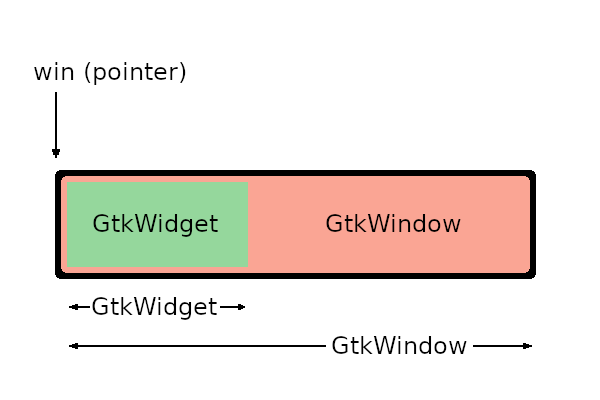
\includegraphics[width=9cm,height=6cm]{../image/window_widget.png}
\caption{GtkWindow and GtkWidget}
\end{figure}

The function \passthrough{\lstinline!gtk\_window\_new!} is defined as
follows.

\begin{lstlisting}[language=C]
GtkWidget *
gtk_window_new (void);
\end{lstlisting}

By this definition, it returns a pointer to GtkWidget, not GtkWindow. It
actually creates a new GtkWindow instance (not GtkWidget) but returns a
pointer to GtkWidget. However,the pointer points the GtkWidget and at
the same time it also points GtkWindow that contains GtkWidget in it.

If you want to use \passthrough{\lstinline!win!} as a pointer to a
GtkWindow type instance, you need to cast it.

\begin{lstlisting}[language=C]
(GtkWindow *) win
\end{lstlisting}

It works, but isn't usually used. Instead,
\passthrough{\lstinline!GTK\_WINDOW!} macro is used.

\begin{lstlisting}[language=C]
GTK_WINDOW (win)
\end{lstlisting}

The macro is recommended because it does not only cast the pointer but
it also checks the type.

\paragraph{Connect it to the
GtkApplication.}\label{connect-it-to-the-gtkapplication.}

The function \passthrough{\lstinline!gtk\_window\_set\_application!} is
used to connect GtkWindow to GtkApplication.

\begin{lstlisting}[language=C]
gtk_window_set_application (GTK_WINDOW (win), GTK_APPLICATION (app));
\end{lstlisting}

You need to cast \passthrough{\lstinline!win!} to GtkWindow and
\passthrough{\lstinline!app!} to GtkApplication with
\passthrough{\lstinline!GTK\_WINDOW!} and
\passthrough{\lstinline!GTK\_APPLICATION!} macro.

GtkApplication continues to run until the related window is destroyed.
If you didn't connect GtkWindow and GtkApplication, GtkApplication
destroys itself immediately. Because no window is connected to
GtkApplication, GtkApplication doesn't need to wait anything. As it
destroys itself, the GtkWindow is also destroyed.

\paragraph{Show the window.}\label{show-the-window.}

The function \passthrough{\lstinline!gtk\_window\_present!} presents the
window to a user (shows it to the user).

GTK 4 changes the default widget visibility to on, so every widget
doesn't need to change it to on. But, there's an exception. Top level
window (this term will be explained later) isn't visible when it is
created. So you need to use the function above to show the window.

You can use
\passthrough{\lstinline!gtk\_widget\_set\_visible (win, true)!} instead
of \passthrough{\lstinline!gtk\_window\_present!}. But the behavior of
these two is different. Suppose there are two windows win1 and win2 on
the screen and win1 is behind win2. Both windows are visible. The
function
\passthrough{\lstinline!gtk\_widget\_set\_visible (win1, true)!} does
nothing because win1 is already visible. So, win1 is still behind win2.
The other function \passthrough{\lstinline!gtk\_window\_present (win1)!}
moves win1 to the top of the stack of the windows. Therefore, if you
want to present the window, you should use
\passthrough{\lstinline!gtk\_window\_present!}.

Two functions \passthrough{\lstinline!gtk\_widget\_show!} and
\passthrough{\lstinline!gtk\_widget\_hide!} is deprecated since GTK
4.10. You should use \passthrough{\lstinline!gtk\_widget\_set\_visible!}
instead.

Save the program as \passthrough{\lstinline!pr3.c!}, then compile and
run it.

\begin{lstlisting}
$ comp pr3
$ ./a.out
\end{lstlisting}

A small window appears.

\begin{figure}
\centering

\includegraphics[width=3.3cm,height=3.825cm]{../image/screenshot_pr3.png}
\caption{Screenshot of the window}
\end{figure}

Click on the close button then the window disappears and the program
finishes.

\subsubsection{GtkApplicationWindow}\label{gtkapplicationwindow}

GtkApplicationWindow is a child object of GtkWindow. It has some extra
feature for better integration with GtkApplication. It is recommended to
use it as the top-level window of the application instead of GtkWindow.

Now rewrite the program and use GtkApplicationWindow.

\begin{lstlisting}[language=C, numbers=left]
static void
app_activate (GApplication *app, gpointer user_data) {
  GtkWidget *win;

  win = gtk_application_window_new (GTK_APPLICATION (app));
  gtk_window_set_title (GTK_WINDOW (win), "pr4");
  gtk_window_set_default_size (GTK_WINDOW (win), 400, 300);
  gtk_window_present (GTK_WINDOW (win));
}
\end{lstlisting}

When you create GtkApplicationWindow, you need to give GtkApplication
instance as an argument. Then it automatically connect these two
instances. So you don't need to call
\passthrough{\lstinline!gtk\_window\_set\_application!} any more.

The program sets the title and the default size of the window. Compile
it and run \passthrough{\lstinline!a.out!}, then you will see a bigger
window with the title ``pr4''.

\begin{figure}
\centering
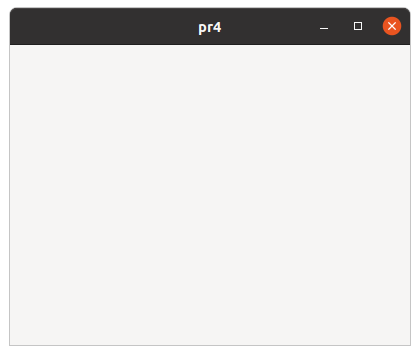
\includegraphics[width=6.3cm,height=5.325cm]{../image/screenshot_pr4.png}
\caption{Screenshot of the window}
\end{figure}
